\documentclass[parskip=half]{scrartcl}

\usepackage[english]{babel}
\usepackage{fontspec}

\usepackage{amsmath}
\usepackage{esvect} % for vectors, way better than \vec
\usepackage{tikz-network}

\newcommand{\definition}[1]{\textsc{#1}}

\renewcommand{\vec}[1]{\vv{#1}}
\newcommand{\mat}[1]{\mathbf{#1}}

\title{The Maths of \emph{Flappy Dragon}}

\begin{document}
\maketitle

\section{Basics}

\subsection{Eggs}
There are various kinds of eggs in the game.
The current Egg \definition{categories} are:
\begin{itemize}
  \item \definition{Rarity}
  \item \definition{Type}
  \item \definition{Subtype}
  \item \definition{Powerup}
  \item \definition{Season}
\end{itemize}

Dragons have different \definition{rarity}, corresponding

\paragraph{Level}
Each time hatching a dragon it gains a \definition{dragon level}.
A dragon's \definition{ability} gets stronger with each level.
The current 

% RARITY    TIME   VALUE  PROBABILITY
% Common     1       40   0.38
% Uncommon   2       80   0.28
% Rare       4      160   0.18
% Epic       8      320   0.09
% Legendary 12      640   0.05
% Mythic    24     1280   0.02


\section{Parameters}
Important Parameters:
\begin{itemize}
\item max dragon level (=10)
\item hatching times
\item mystery egg probabilities
\item egg value factor ($40 \cdot 2^{\textrm{rarity-rank}}$)
\item max affinity
\end{itemize}

andere Begriffe:

dragon
tower
score
crowns
aristocrat / royal : the game says aristocrat, but the code uses royal (shorter, easier to type)
treasure chests
eggs
to hatch an egg in the nest screen
skills (active with cooldown \& passive with condition) / ability
skill level (increased by getting duplicate dragons)
stats (=weight,force,speed)
controls (=tap,hold,follow,reverse-)
powerups provide effects
  Dragon heart
  Suspicious mushroom
  Fairy dust
  Dragon eye
  Dragon chilli
  Thundercloud
  Sands of time
  Cosmic stars
  Lucky charm
  Curved spoon
  Magic snowflake
  Spooky ghost
Mystery egg : found in-game or bought at shop (fixed crown price)
Stellar donut
  normal: level up a dragon
  shiny:
  powerup
Dimensional Rift / Portal
Store: buy eggs
Lair: breed a couple/pair of dragons to generate eggs
Affinity [to get shiny eggs)
Nest: Hatch dragon eggs
Mastery
Quests


\section{Probability of items}
When generating a new tower, how likely will it have a chest/powerup/aristocrat/…?

The game code does not have absolute probabilities, but relative \emph{weights} $w_i$.
This makes the condition $\sum p_i = 1$ easier to implement.
The absolute probability $p_x$ of an item $x$ can be calculated relative to the total weight of all items:
\[ p_x = \frac{w_x}{\sum_{i \in I} w_i} \]

All the items which can appear on towers are:
\begin{itemize}
  \item nothing
  \item royal (aristocrat)
  \item chest
    \begin{itemize}
      \item woodchest
      \item ironchest
      \item goldchest
      \item diamondchest
      \item pumpkinchest
      \item presentchest
    \end{itemize}
  \item powerup
    \begin{itemize}
      \item dragonheart
      \item suspiciousmushroom
      \item fairydust
      \item dragoneye
      \item dragonchilli
      \item thundercloud
      \item sandsoftime
      \item cosmicstars
      \item luckycharm
      \item curvedspoon
      \item magicsnowflake
      \item spookyghost
    \end{itemize}
  \item portal
  \item donut
\end{itemize}

Table of items and their weights:

\begin{tabular}{lr}
  Nothing & 1000 \\
  Aristocrat & 500 \\
  Chest & 250 \\
  Powerup & 150 \\
  Egg & 25 \\
  Rift & 18 \\
  Donut & 12\\
\end{tabular}

The \emph{Lucky Charm} powerup modifies the base weights as follows:

\begin{tabular}{lrr}
  Nothing & 1000 & $\times 0$ \\
  Royal & 500 & $\times 1$ \\
  Chest & 250 & $\times 5$ \\
  Powerup & 150 & $\times 1$ \\
  Egg & 25 & $\times 5$ \\
  Portal & 18 & $\times 1$ \\
  Donut & 12 & $\times 5$ \\
\end{tabular}

Chests also work with a weight-based system:

\begin{tabular}{lrr}
  Chest   & Weight & Crowns \\
  \hline
  Wood    & 50 & 1--3 \\
  Iron    & 30 & 2--4 \\
  Gold    & 15 & 3--5 \\
  Diamond &  5 & 4--6 \\
  Pumpkin &  5 & 1--6 \\
  Present &  5 & 1--6 \\
\end{tabular}

\subsection{Lucky state, Markov chains}
Haben eine FSM (finite state machine), endl. Zustandsautomaten mit $n$ Zuständen.
Die Übergangswahrscheinlichkeiten erfasst in Matrix $M$ (quadratisch) mit Einträgen $p_{ij}$, beschreibt WSK des Übergangs $i \rightarrow j$.
Die Zeilensummen sind je $1$ (alle $i$ verlassenden). Die Spaltensummen sind je $1$ (alle in $j$ eingehenden).

Die Gesamtwahrscheinlichkeit $p_j^{(t+1)}$, im nächsten Zeit-Schritt $t+1$ den Zustand $j$ zu erreichen, ist demnach
\[ p_j^{(t+1)} = p_1^{(t)}p_{1,j} + p_2^{(t)}p_{2,j} + \dots +  p_n^{(t)}p_{n,j} = \sum_{i=1}^n p_i^{(t)}p_{i,j} \]

\[ \vec{p^{(t)}} = \begin{pmatrix}p_1 & p_2 & \dots & p_n \end{pmatrix}^{(t)} \]

Das ist eine Matrixmultiplikation, deshalb muss $p$ (bzw. $\pi$) ein Zeilenvektor sein:
\[ (p(1) p(2) \dots p(n)) = p \cdot M = p\prime \]
(wsk Zustände erster Schritt zu WSK Zustände nächster Schritt)
alternativ Matrix transponieren.

Für den Gleichgewichtszustand (stationäre Verteilung, engl. (stationary/steady state) distribution) Equilibrium muss dann gelten:
\[ \pi \mathrm{M} = \pi \]

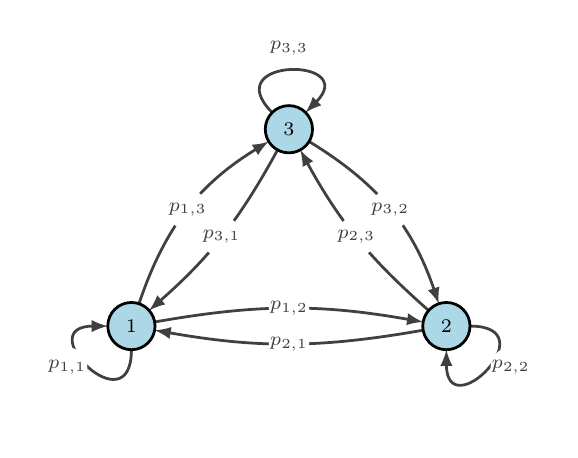
\begin{tikzpicture}
  \Vertex[label=1]{1}
  \Vertex[label=2,x=4]{2}
  \Vertex[label=3,x=2,y=2.5]{3}

  \Edge[Direct,label=$p_{1,2}$,lw=1pt,bend=10](1)(2)
  \Edge[Direct,label=$p_{2,1}$,lw=1pt,bend=10](2)(1)

  \Edge[Direct,label=$p_{1,3}$,lw=1pt,bend=20](1)(3)
  \Edge[Direct,label=$p_{3,1}$,lw=1pt,bend=10](3)(1)

  \Edge[Direct,label=$p_{2,3}$,lw=1pt,bend=10](2)(3)
  \Edge[Direct,label=$p_{3,2}$,lw=1pt,bend=20](3)(2)

  % selfloops
  \Edge[Direct,label=$p_{1,1}$,lw=1pt,bend=20,loopposition=225,position=left](1)(1)
  \Edge[Direct,label=$p_{2,2}$,lw=1pt,bend=20,position=right,loopposition=-45](2)(2)
  \Edge[Direct,label=$p_{3,3}$,lw=1pt,bend=20,loopposition=90,position=above](3)(3)

\end{tikzpicture}

Dieser Zustandsgraph führt zur folgenden Matrix, deren Einträge $p_{i,j}$ die jeweilige Übergangswahrscheinlichkeit von Zustand $i$ nach Zustand $j$ beschreiben:
\[ \mat{M} = 
\begin{pmatrix}
  p_{1,1} & p_{1,2} & p_{1,3} \\
  p_{2,1} & p_{2,2} & p_{2,3} \\
  p_{3,1} & p_{3,2} & p_{3,3}
\end{pmatrix}
\]

Es ist
$
\vec{p}^{(t+1)}
= \vec{p}^{(t)}\cdot\mat{M}
= \vec{p^{(t-1)}}\cdot\mat{M}^2 = \dots
= \vec{p}^{(0)}\cdot\mat{M}^{t}
$

Falls es ein Gleichgewicht/Equilibrium/stationäre Verteilung $\vec{p^*}$ gibt, so muss für diese gelten
\[ p^*\mat{M} = p^* \]
Vergleiche mit der Definition von (linken) Eigenvektoren:
\[ \vec{v}\mat{A} = \lambda \vec{v} \]

dh. der linke EV zu $\lambda=1$ ist eine Lösung.

Danach muss noch normiert werden (damit $\sum p = 1$): \[ p = \frac{\vec{v}}{\sum\vec{v}} \]

% Testbild für tikz-network
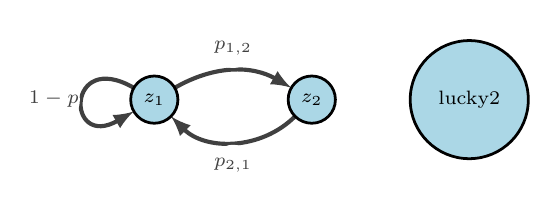
\begin{tikzpicture}
  \Vertex[label=$z_1$]{A}
  \Vertex[x=2,label=$z_2$]{B}
  \Vertex[x=4,label=lucky2,shape=circle,size=1.5]{C}
  \Edge[bend=30,label=$p_{1,2}$,position=above,Direct](A)(B)
  \Edge[Direct,loopposition=180,loopshape=-60,label=$1-p$,position=left](A)(A)
  \Edge[bend=45,Direct,label=$p_{2,1}$,position=below](B)(A)
\end{tikzpicture}

\subsubsection{Zustandsgraph/Matrix für Lucky Charm Powerup}
Wie funktioniert das …?
Der Lucky-Zustand („Glückszustand“?) hält – je nach konkretem Drachen – bis zu $l$ Türme an\footnote{eigentlich 12 Sekunden, aber jeder Drache hat andere Geschwindigkeit. Da wir uns sowieso nur für die Anzahl der Türme interessieren, die in dieser Zeit durchflogen werden, können wir das auch diskretisieren}; bekommt man in dieser Zeit aber erneut ein Lucky Charm, wird dieser Zähler zurückgesetzt (nicht addiert).

Zustandsgraph für $l=4$

\begin{figure}
  \centering
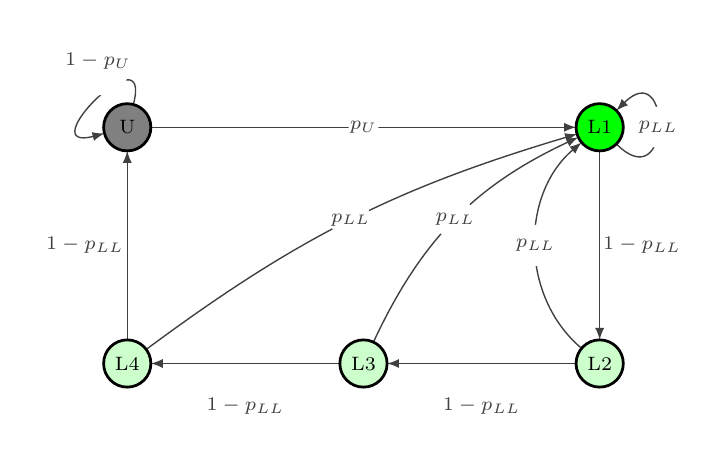
\begin{tikzpicture}
  \SetDistanceScale{3}
  \SetVertexStyle[ Shape=circle ]
  \SetEdgeStyle[LineWidth=0.5pt ]
  \Vertex[x=0,y=0,  label=U,  color=gray]{U}
  \Vertex[x=2,y=0,  label=L1, color=green]{L1}
  \Vertex[x=2,y=-1, label=L2, color=green,opacity=0.2]{L2}
  \Vertex[x=1,y=-1, label=L3, color=green,opacity=0.2]{L3}
  \Vertex[x=0,y=-1, label=L4, color=green,opacity=0.2]{L4}

  \Edge[Direct, loopposition=135, loopshape=-120, position=above, label=$1-p_U$](U)(U)
  \Edge[Direct, loopposition=0, loopshape=-90, label=$p_{LL}$](L1)(L1)
  \Edge[Direct, label=$p_U$](U)(L1)
  \Edge[Direct, position=right, label=$1-p_{LL}$](L1)(L2)
  \Edge[Direct, position=below, label=$1-p_{LL}$](L2)(L3)
  \Edge[Direct, position=below, label=$1-p_{LL}$](L3)(L4)
  \Edge[Direct, position=left,  label=$1-p_{LL}$](L4)(U)

  \Edge[Direct, bend=50, label=$p_{LL}$](L2)(L1)
  \Edge[Direct, bend=20, label=$p_{LL}$](L3)(L1)
  \Edge[Direct, bend=10, label=$p_{LL}$](L4)(L1)
\end{tikzpicture}
  \caption{transition diagram for 4 lucky states}
\end{figure}

This leads to the transition matrix
for $p=\begin{pmatrix}U & L1 & L2 & L3 & L4 \end{pmatrix}$
\[ \mat{P}=\begin{pmatrix}
  % U L1 L2 L3 L4
  1-p_U & p_U & 0 & 0 & 0 \\% U
    0 & p_L & 1-p_L & 0 & 0 \\% L1
    0 & p_L & 0 & 1-p_L & 0 \\ % L2
    0 & p_L & 0 & 0 & 1-p_L \\   % L3
  1-p_L & p_L & 0 & 0 & 0 \\   % L4
\end{pmatrix}
\]

\end{document}
